\chapter{Indroduction to chaotic dynamics}
We begin with a few motivating examples.
\begin{ex}[Periodically forced slender beam]
	A beam is hanging on the inside of a rectangular frame, attached to the upper edge. Two permanent magnets are attached to the lower edge. Furthermore, there is a $T=2 \pi $-periodic forcing in the horizontal direction to the frame. The deflection of the beam is measured by the variable $x$. The setup is illustrated in Fig. \ref{fig:forced_slender_beam}.
	\begin{figure}[h!]
		\centering
		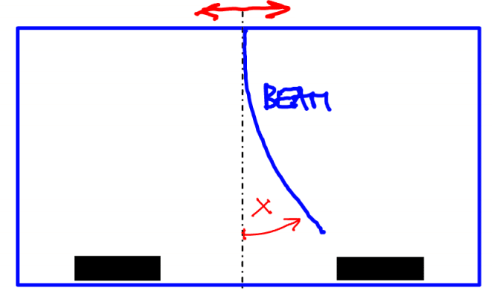
\includegraphics[width=0.5\textwidth]{figures/ch6/1forced_slender_beam.png}
		\caption{Depiction of the periodically forced slender beam. The frame is given by the blue rectangle. The two permanent magnets are represented by the black boxes.}
		\label{fig:forced_slender_beam}
	\end{figure}
This leads to the equation of motion
\begin{align}
	\ddot{x} + \dot{x} - x + x^3 = \varepsilon \cos(t);\quad 0 \leq \varepsilon \ll 1.
\end{align}
Therefore we have a perturbed Duffing oscillator. We transform the system into a first order ODE
\begin{align}
	\begin{dcases}
		\dot{x} = y \\
		\dot{y} = -y +x - x^3 + \varepsilon \cos(t).
	\end{dcases}
\end{align}
For $\varepsilon =0$ damping, two homoclinic orbits arise for the three fixed points. However, for nonzero damping, we get seemingly chaotic behavior. Both of these regimes are depicted in Fig. \ref{fig:pert_duffing}.
\begin{figure}[h!]
	\centering
	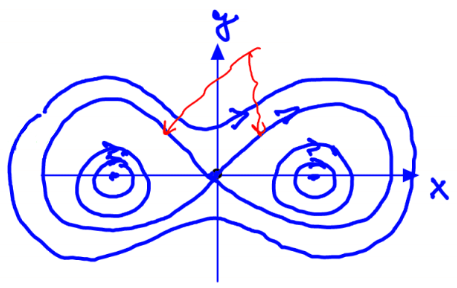
\includegraphics[width=0.45\textwidth]{figures/ch6/3unpert_duffing.png}
	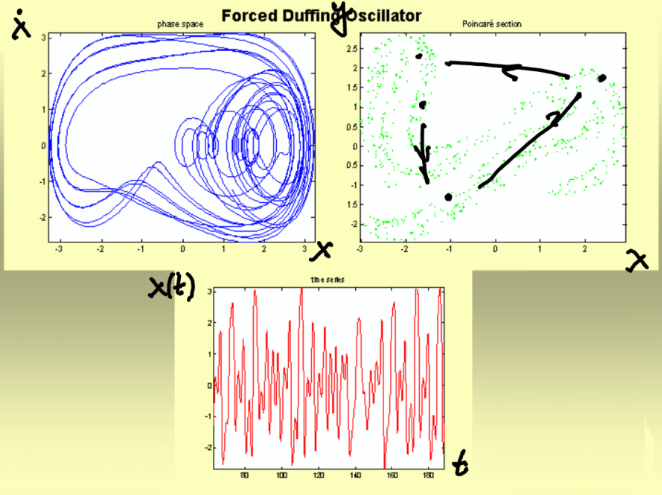
\includegraphics[width=0.45\textwidth]{figures/ch6/2pert_duffing.png}
	\caption{Left: Duffing oscillator with $\varepsilon=0$ damping, the red arrows designate the homoclinic orbits. Right: (Clockwise from top left) The phase space of the (nonzero) perturbed Duffing oscillator; The Poincaré section of the damped Duffing oscillator, with the Poincaré map illustrated by the black arrows; The value of $x(t)$ over time, with no apparent pattern.}
	\label{fig:pert_duffing}
\end{figure}

\end{ex}

\begin{ex}[2-dimensional Rayleigh-Bernard convection]
	A fluid is held between two plates. The upper plate is cold and the lower plate is hot. This causes convections to form as hotter fluid rises and colder fluid falls. So called convection cells then form for low Rayleigh numbers. This process is illustrated in Fig. \ref{fig:convection_cells}.
	\begin{figure}[h!]
		\centering
		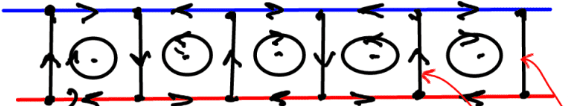
\includegraphics[width=0.65\textwidth]{figures/ch6/4convection_plates.png}
		\caption{Convection cells forming between two plates of different temperature. The cold plate (blue) is vertically above the hot plate (red). Each black dot represents a fixed point of the system, with heteroclinic orbits connecting them (red arrows). This is in an unperturbed setting ($\varepsilon =0 $).}
		\label{fig:convection_cells}
	\end{figure}

	If the Rayleigh number $R_{a}$ exceeds a critical value $R_{a_{ \textrm{crit} }}$, we have a time periodic perturbation to the velocity field. The fluid trajectories have the following equations of motion
	\begin{align}
		\begin{dcases}
			\dot{x} = u(x,y) + \varepsilon u_1(x,y,t) \\
			\dot{y} = v(x,y) + \varepsilon v_1 (x,y,t)
		\end{dcases}
;\quad \varepsilon>0.		
	\end{align}
	Here, the functions $u_1$ and $v_1$ are $T$-periodic. The chaotic nature of this system is shown in Fig. \ref{fig:convection_chaos}.
	\begin{figure}[h!]
		\centering
		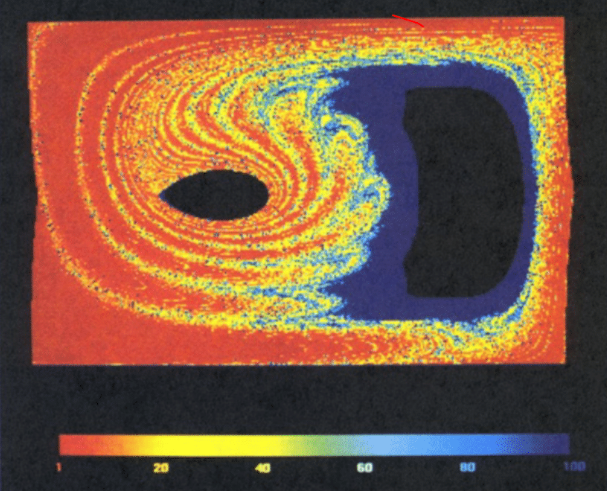
\includegraphics[width=0.4\textwidth]{figures/ch6/5convection_chaos.png}
		\caption{Escape time from one convection cell. The number of iterations of the Poincaré map needed for escape is given by the color scale. Here $0 < \varepsilon \leq 1$.}
		\label{fig:convection_chaos}
	\end{figure}
	
\end{ex}

Moving forward we will have a common mathematical setting
\begin{align}
	\dot{x} = f(x) + \varepsilon g(x,t);\quad x \in \mathbb{R}^{2},\quad g(x,t) =g(x,t+T);\quad 0 \leq \varepsilon \ll 1;\quad f,t\in C^{1}. \numberthis \label{eq7:one}
\end{align}
We have a small $T$-periodic perturbation of a planar ODE which can be studied via a Poincaré map $P_{\varepsilon}^{t_0}:x_0 \mapsto x(t_0 + T; t_0,x_0)$. Assume that for $\varepsilon=0$ the system \eqref{eq7:one} has a saddle type fixed point with a homoclinic (or heteroclinic) orbit $x^{0}(t-t_0)$. Such a system is depicted in Fig. \ref{fig:assumptions}.
\begin{figure}[h!]
	\centering
	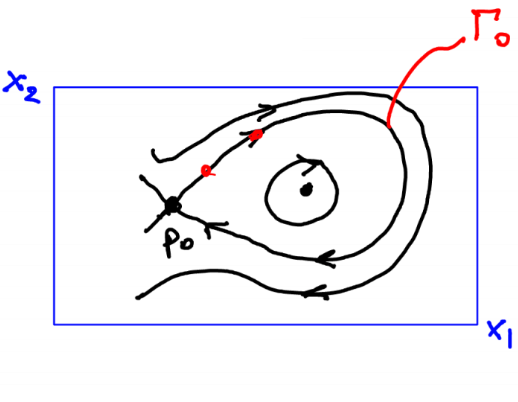
\includegraphics[width=0.45\textwidth]{figures/ch6/6assumptions_a.png}
	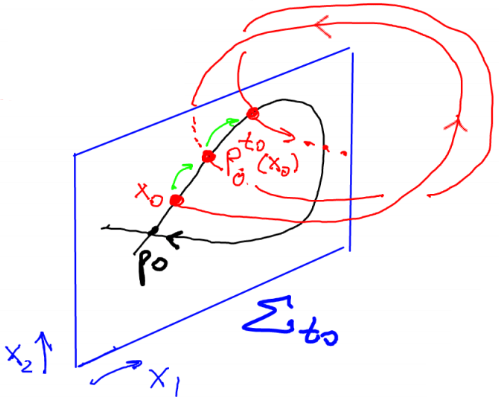
\includegraphics[width=0.45\textwidth]{figures/ch6/7assumptions_b.png}
	\caption{Left: An example of a system following the assumptions. The homoclinic orbit $\Gamma_0$ is equal to the local unstable and local stable manifolds. Right: The Poincaré map for $\varepsilon=0$, with time running counterclockwise about the $x_1$ axis with period $T$.}
	\label{fig:assumptions}
\end{figure}

\begin{remark}[]
	The fixed point of $P_{0}^{t_0}$ given by $p_0 $ is hyperbolic
	\begin{align}
	P_{0}^{t_0}(p_0) = p_0;\quad DP_{0}^{t_0}(p_0)  \textrm{ has eigenvalues }  \lambda_1,\lambda_2:\ |\lambda _1|<1,\ |\lambda _2|>1.
	\end{align}
	
\end{remark}

More generally we define a hyperbolic fixed point for a map.
\begin{definition}
	For a map $F:\mathbb{R}^{n}\to \mathbb{R}^{n}$ and a dynamical system with $x_{k+1} = F(x_k)$, the fixed point $p_0$ (i.e. $F(p_0) = p_0 $) is \emph{hyperbolic} if the linearization's $DF(p_0)\in \mathbb{R}^{n\times n}$ eigenvalues $\lambda_1,\ldots,\lambda_n $ never have unitary length: $|\lambda_i| \neq 1$ for $i=1,\ldots,n$.
\end{definition}

For each eigenvalue $\lambda _i$ of the linearization the corresponding eigenvector is given by $s_i$. Assume that $DF(p_0)$ is semisimple, i.e. all of the eigenvectors are linearly independent. The linearized dynamics at $p_0$ for $y=x-p_0$ small are
\begin{align}
	y_{k+1} = DF(p_0)y_k \implies y_k = \lambda_1^{k} c_1 s_1 + \ldots + \lambda_n^{k} c_n s_n.	
\end{align}
If all of the eigenvalues have less than unitary magnitude, $|\lambda _i|<1$ for $i=1,\ldots,n$, then $p_0$ is asymptotically stable. Otherwise if there exists an eigenvalue with norm strictly larger than 1, $p_0$ is unstable. The relationship of the nonlinear and linearized dynamics are shown in Fig. \ref{fig:lin_nonlin_relation}.
\begin{figure}[h!]
	\centering
	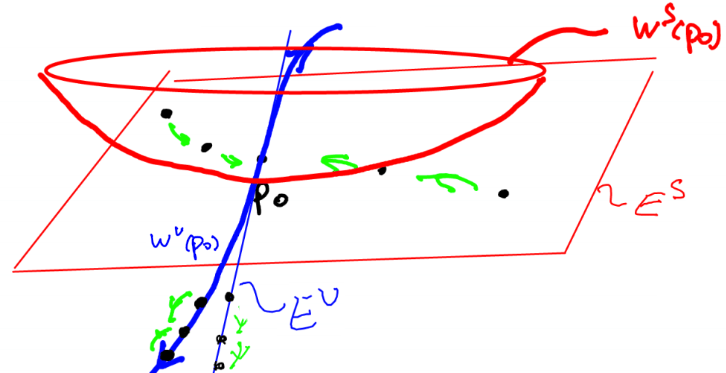
\includegraphics[width=0.65\textwidth]{figures/ch6/9lin_nonlin_relationship.png}
	\caption{The stable ($W^{S}(p_0)$) and unstable ($W^{U}(p_0)$) manifolds drawn in relation to the stable ($E^{S}$) and unstable ($E^{U}$) subspaces. The subspaces are given as the span of the stable (resp. unstable) eigenvectors. The green arrows signify steps of the linearized (resp. original) system.}
	\label{fig:lin_nonlin_relation}
\end{figure}

The fixed point $p_0$ along with the stable and unstable manifolds ($W^{S}(p_0)$ and $W^{U}(p_0)$) persist smoother under small smooth perturbations to $F$ near $p_0$.

\section{Consequences of hyperbolicity}
Hyperbolicity has a few important consequences in our setting. Foremost, the perturbed hyperbolic fixed point $p_{\varepsilon}^{t_0}$ has a hyperbolic periodic orbit for the ODE.Furthermore, the solutions of the ODE are smooth in $\varepsilon$, thus the solutions within $W^{U}(p_{\varepsilon}^{t_0})$ and $W^{S}(p_{\varepsilon}^{t_0})$ remain $\mathcal{O}(\varepsilon)$ close to $\Gamma_0$, i.e.

\begin{align}
	x_{\varepsilon}^{S}(t;t_0) &= x^{0}(t-t_0) + \varepsilon a^{S}(t) + \mathcal{O}(\varepsilon^{2} );\quad t\in [t_0,\infty ) \\
	x_{\varepsilon}^{U}(t;t_0) &= x^{0}(t-t_0) + \varepsilon a^{U}(t) + \mathcal{O}(\varepsilon^{2} );\quad t\in (-\infty, t_0].
\end{align}

Now we examine what the global shape of these manifolds are for $\varepsilon>0$ and if they interact. To do this we will follow an idea from Poincaré, Arnold, and Melnikov. To this end we define the perpendicular to $f$ 
\begin{align}
	f^{\perp}(x^{0}(0)) = 
	\begin{pmatrix}
		-f_2(x^{0}(0)) \\ f_1 (x^{0}(0))
	\end{pmatrix}
	.
\end{align}
We would like to use this to measure the distance between $x^{U}_{\varepsilon}(t_0;t_0)$ and $x^{S}_{\varepsilon}(t_0;t_0)$. The outlook for this is shown in Fig. \ref{fig:PAM_idea}.
\begin{figure}[h!]
	\centering
	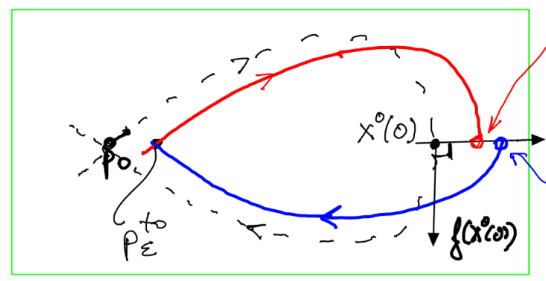
\includegraphics[width=0.5\textwidth]{figures/ch6/10PAM_idea.png}
	\caption{The Poincaré-Arnold-Melnikov idea. The dotted black line signifies $\Gamma$, the red dot $x^{U}_{\varepsilon}(t_0;t_0)$, the blue dot $x^{S}_{\varepsilon}(t_0;t_0)$, and the arrow pointing to the right $f^{\perp}$. The plane is $\Sigma_{t_0}$.}
	\label{fig:PAM_idea}
\end{figure}
Thus we have a signed distance function
\begin{align}
	d_{\varepsilon}(t_0) = \frac{\left\langle f^{\perp}(x^{0}(0)), x^{U}_{\varepsilon(t_0; t_0) - x^{S}_{\varepsilon}(t_0; t_0)}\right\rangle}{\left| f^{\perp}(x^{0}(0))\right|} 
	= \varepsilon  \frac{\left\langle f^{\perp}(x^{0}(0)), a^{U}(t_0) - a^{S}(t_0) \right\rangle}{\left| f^{\perp}(x^{0}(0))\right|} + \mathcal{O}(\varepsilon^2).
\end{align}
The numerator in the second equation is called the \emph{Melnikov function}
\begin{align}
	M(t_0)=\left\langle f^{\perp}(x^{0}(0)), a^{U}(t_0) - a^{S}(t_0) \right\rangle	.
\end{align}
In fact Melnikov proved an identity for this function.
\begin{theorem}[Melnikov]
	\begin{align}
		M(t_0) = \int_{-\infty }^{\infty }  \langle f^{\perp}(x^{0}(t-t_0)), g(x^{0}(t-t_0),t)\rangle dt.
	\end{align}
	For the proof, see the book by Guckenheimer \& Holmes.	
\end{theorem}
\begin{remark}[]
	The integral in Melnikov's theorem converges as $|g(x^{0}(t-t_0),t)|$ is globally bounded as $t \to \pm \infty $ and $|f^{\perp}| = |f|$ and
	\begin{align}
		\lim_{t\to \pm \infty }\left| f(x^{0}(t-t_0)) \right| =0,
	\end{align}
	exponentially as $p_0$ is a hyperbolic fixed point.	
\end{remark}

\begin{remark}[]
	In order to evaluate $M(t_0)$ we do not need to solve the perturbed ODE $\dot{x} =f(x) + \varepsilon g(x,t)$, instead we only need $x^{0}(t-t_0)$.
\end{remark}

Now observe that
\begin{align}
	d_{\varepsilon} (t_0) = 0 \iff \varepsilon \frac{M(t_0)}{\left| f^{\perp}(x^{0}(0))\right|} + \mathcal{O}(\varepsilon^2) = 0 \overset{\varepsilon \neq 0}{\iff} \underbrace{\frac{M(t_0)}{\left| f^{\perp}(x^{0}(0)) \right|} + \mathcal{O}(\varepsilon)=0}_{F(t_0, \varepsilon) = 0}.
\end{align}
Now we would like to know when we can find a solution $t_0(\varepsilon)$ such that $d_{\varepsilon}(t_0(\varepsilon))=0$ for $\varepsilon > 0$. To do this we use the Implicit Function Theorem. First assume that $F(\overline{t}_{0}, 0) = 0$, i.e. $M(\overline{t}_0) = 0$, and $\frac{\partial F}{\partial t_0}(\overline{t}_0), 0) \neq 0$, i.e. $\frac{\partial }{\partial t_0}M(\overline{t}_0) \neq 0$. If this condition is fulfilled the root is called \emph{transverse}.  Then there exists a unique $t_0(\varepsilon) = \overline{t}_{0} + \mathcal{O}(\varepsilon)$ which solves $F(t_0(\varepsilon), \varepsilon)=0$ for $\varepsilon \neq 0$ small enough. Also $t_0(\varepsilon)$ is smooth if $F(t_0,\cdot)$ is smooth.

A transverse zero for $M(t_0)$ implies that the Melnikov distance $d_{\varepsilon }(t_{0}(\varepsilon)=0$, in turn implying that the intersection of the stable and unstable manifolds have a nonzero intersection, $W^{S}(p_{\varepsilon}^{t_0}) \cap W^{U}(p_{\varepsilon}^{t_0}) \neq \emptyset$. Therefore we have an element $q\in W^{S}(p_{\varepsilon}^{t_0}) \cap W^{U}(p_{\varepsilon}^{t_0})$, for this $q$ we also have that for every $n \in \mathbb{Z}$
\begin{align}
	P_{\varepsilon}^{n}(q) \in W^{S}(p_{\varepsilon}^{t_0}) \cap W^{U}(p_{\varepsilon}^{t_0}). 
\end{align}
Therefore we have that for each iterate of the Poincaré map there is a unique point in both the stable and unstable manifolds, so these must intersect each other infinitely many times. This behavior is shown in Fig. \ref{fig:inf_intersections}. 
\begin{figure}[h!]
	\centering
	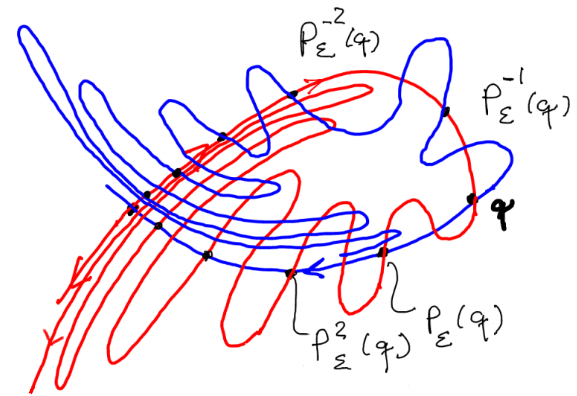
\includegraphics[width=0.45\textwidth]{figures/ch6/11inf_intersection_hetero.png}
	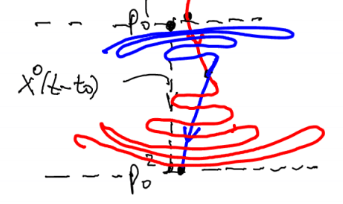
\includegraphics[width=0.45\textwidth]{figures/ch6/11inf_intersection_homo.png}
	\caption{The infinite intersections of the stable and unstable manifolds for a transitive zero. Left: The homoclinic case, this is aptly called a \emph{homoclinic tangle}. Right: The heteroclinic case.}
	\label{fig:inf_intersections}
\end{figure}
In the homoclinic tangle, we can see the accumulation of trajectories that are caused by the accumulation of the iterates of the Poincaré map. {\color{blue} He says to see the $\Lambda$ lemma, not sure exactly what is meant by that.}

\begin{remark}[]
	It is impossible for stable and unstable manifolds to intersect themselves. This is usually argued by stating that $q$ cannot have two distinctive preimages under a diffeomorphism. However, this is not sufficient as a self intersection does not imply that two distinct preimages exist, for instance a loop de loop manifold structure and suitable Poincaré map as in Fig. \ref{fig:loopdeloop}.
	\begin{figure}[h!]
		\centering
		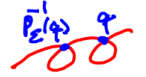
\includegraphics[width=0.25\textwidth]{figures/ch6/12loopdeloop.png}
		\caption{An example for a self-intersecting manifold without $q$ having multiple preimages.}
		\label{fig:loopdeloop}
	\end{figure}
A priori, this is possible to occur. In this case the existence of one loop actually implies the existence of infinitely many converging to $p_{\varepsilon}$. Thereby there must exist a loop in every arbitrarily small neighborhood of $p_{\varepsilon}$, this then contradicts the Hartman-Grobman Theorem as our system must be topologically equivalent to the linear saddle in a small enough neighborhood. 	
\end{remark}

\begin{remark}[]
	For every pair of intersections $P_{\varepsilon}^{k}(q)$ and $P _{\varepsilon}^{k+1}(q)$, there exists at least another intersection between the stable and unstable manifolds. This is due to the fact that $P_{\varepsilon}$ is orientation preserving (i.e. $DP_{\varepsilon}(q)$ is an orientation preserving linear map). The implication here is illustrated in Fig. \ref{fig:between_intersections}.
\begin{figure}[h!]
	\centering
	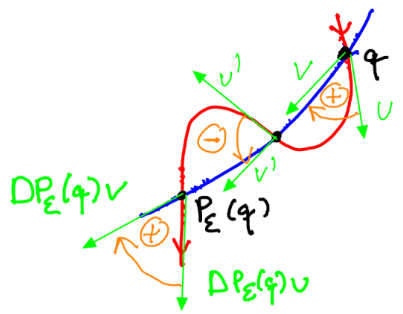
\includegraphics[width=0.5\textwidth]{figures/ch6/13between_intersections.png}
	\caption{Another intersection of the stable and unstable manifolds exists between two sequential iterates of the Poincaré map due to the preservation of orientation under this map.}
	\label{fig:between_intersections}
\end{figure}

The orientation preserving nature of $P_{\varepsilon}$ can be seen by using Liouville's Theorem 
	\begin{align}
		\det(DF_{t_0}^{t}(p)) = \exp \left( \int_{t_0}^{t}  \textrm{div}  ( f(x(s;t_0,p),s))ds\right),
	\end{align}
	for the flow map $F_{t_0}^{t}:x_0 \mapsto x(t;t_0,x_0)$	of the dynamical system $\dot{x} = f(x,t)$. In our case we find
	\begin{align}
		\det (DP_{\varepsilon}(q)) = \exp\left(\int_{t_0}^{t}  \textrm{div} \left. (f + \varepsilon g) \right|_{x_{\varepsilon}(t);\ x_{\varepsilon}(t_0)=q}) ds \right) > 0
	\end{align}
	Therefore $DP_{\varepsilon}(q)$ is orientation preserving, in fact Poincaré maps in general are orientation preserving.	
\end{remark}

\begin{ex}[The forced-damped Duffing equation]
Recall the dynamical system
\begin{align}
	\begin{dcases}
		\dot{x}=y \\
		\dot{y} = x - x^3  + \varepsilon ( \gamma \cos(\omega t) -\delta y)
	\end{dcases}
	;\quad |\varepsilon|\ll 1.
\end{align}
Here the forcing amplitude is given by $\gamma $ and the linear damping coefficient by $\delta $. We separate the right hand side into two parts
\begin{align}
	f(x,y) = 
	\begin{pmatrix}
		y \\ x - x^3
	\end{pmatrix},\quad
	g(x,y) =
	\begin{pmatrix}
	0 \\  \gamma \cos(\omega t) -\delta y
	\end{pmatrix}
	. \numberthis \label{eq7:juan}
\end{align}
A Hamiltonian for this system is given by 
\begin{align}
	H = \frac{1}{2}y^2 - \frac{1}{2} x^2  + \frac{1}{4}x^4 = E_{0} =  \textrm{const} .
\end{align}
Further the phase portrait for $\varepsilon=0$ is known and shown in Fig. \ref{fig:duffing_phase}. {\color{blue} He has $\varepsilon>0$ in the script, pg 12, but I think that is wrong.}
\begin{figure}[h!]
	\centering
	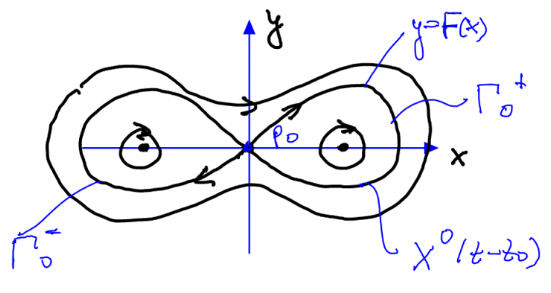
\includegraphics[width=0.5\textwidth]{figures/ch6/14duffing_phase.png}
	\caption{The phase portrait for the forced-damped Duffing oscillator for $\varepsilon=0.$}
	\label{fig:duffing_phase}
\end{figure}
We have that locally $\dot{x}=F(x)$, thus we have a separable equation. Colloquially this can be seen as follows (the implication is not rigorous and should not be interpreted as usual)
\begin{align}
	\frac{dx}{dt} = F(x) \implies \int_{0}^{x}  \frac{d \tilde{x}}{F(\tilde{x})} = \int_{0}^{t} d \tilde{t}.
\end{align}
Hence, on $\Gamma_{0}^{+}$, we have 
\begin{align}
	x_0(t) = 
	\begin{pmatrix}
		\sqrt{2}  \textrm{sech}(t) \\  -\sqrt{2}  \textrm{sech} (t) \tanh(t)
	\end{pmatrix}
.	
\end{align}
Now for $\varepsilon>0$ we calculate the Melnikov function
\begin{align}
	M^{+}(t_0) &= \int_{-\infty }^{\infty }\langle f^{\perp}(x^{0}(t-t_0), g(x^{0}(t-t_0), t) \rangle dt \\
		   &= - \frac{4 \delta }{3} + \sqrt{2} \gamma \pi \omega  \textrm{sech} \left( \frac{\pi \omega }{2}\right)\sin(\omega t_0). 
\end{align}
Next, we ask if this is equal to zero and look for a transverse zero. To this end we define $R^{0}(\omega) = \frac{4 \cosh \left( \frac{\pi \omega }{2}\right)}{3 \sqrt{2} \pi \omega }$. Thus the zeros of the Melnikov function are given by
 \begin{align}
	 R^{0}(\omega) = \frac{\gamma }{\delta} \sin(\omega t_0).
\end{align}
{\color{blue} I wasn't sure how he got the graph and what the marks meant, so I thought it wouldn't be clear to students, so I tried to do this part myself. I get the inverse result of him}.
A solution is then a transitive zero if the partial derivative with respect to $t_0$ is nontrivial
\begin{align}
	\sqrt{2} \gamma \pi  \omega ^2  \textrm{sech} \left( \frac{\pi \omega }{2}\right) \cos(\omega t_0) \neq 0
\end{align}
The $ \textrm{sech} $ function is nonzero, thus we only need to know when $\cos(\omega t_0)=0$, which occurs for $\omega t_0 = (2k+1)\pi $, or as a function of $t_0$ when $\frac{\omega }{\pi } = \frac{2k+1}{t_0}$. Thus at the odd integers scaled by $\frac{1}{t_0}$, we have nontransverse zeros, and all other roots of the Melnikov function are transverse. This is depicted in Fig. \ref{fig:beam_tangle}.
\begin{figure}[h!]
	\centering
	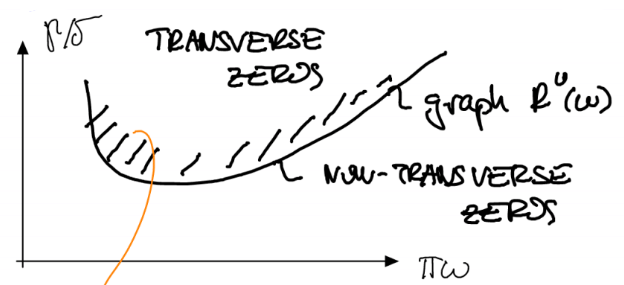
\includegraphics[width=0.6\textwidth]{figures/ch6/15beam_tangle.png}
	\caption{The yellow line showing that a homoclinic tangle exists for the forced-damped Duffing oscillator.}
	\label{fig:beam_tangle}
\end{figure}
{\color{blue} We need to go over this part I think.}
\end{ex}

\section{Dynamics near the homoclinic tangle \& Smale's horseshoe map}
We now continue and examine the dynamics near the homoclinic tangle. Consider the dynamical system
\begin{align}
	\dot{x} = f(x) + \varepsilon g(x,t);\quad x \in \mathbb{R}^{2};\quad f,g \in  \mathcal{C}^{1};\quad g(x,t) = g(x,t+T).
\end{align}
{\color{blue} Here I used mathcal\{C\} instead of C, I like this, think we should do it everywhere}
After an appropriate change of coordinates we find the geometry called \emph{Smale's construction}, which is as shown as in Fig. \ref{fig:smales_construction}.
\begin{figure}[h!]
	\centering
	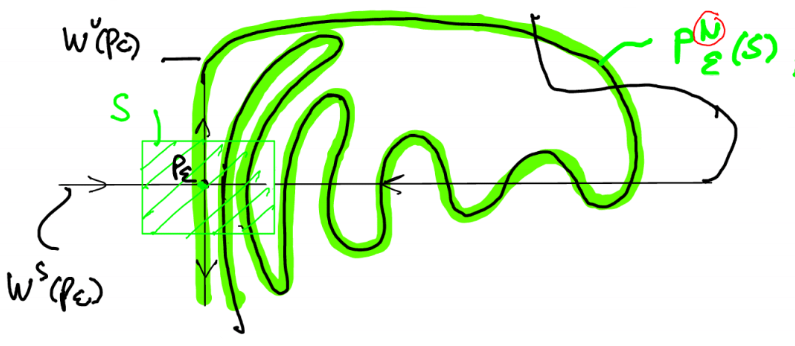
\includegraphics[width=0.7\textwidth]{figures/ch6/16smales_construction1.png}
	\hspace{0.03\textwidth}
	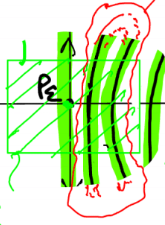
\includegraphics[width=0.25\textwidth]{figures/ch6/16smales_construction2.png}
	\caption{Smale's construction is found through an appropriate change of coordinates. Left: The full construction, the $N$ circled in red is large enough such that $P^{N}_{\varepsilon}(S)\cap S = \emptyset$, where $S$ is the green rectangle around $p_{\varepsilon}$. Right: Focus on the set $S$, the red lines designate a horseshoe-like structure.}
	\label{fig:smales_construction}
\end{figure}


